\documentclass[a4paper,12pt]{article}
\usepackage[utf8]{inputenc}
\usepackage{geometry}
\usepackage{titlesec}
\usepackage{listings}
\usepackage{xcolor}
\usepackage{pgfplots}
\usepackage{float}

\geometry{top=2.5cm, bottom=2.5cm, left=2.5cm, right=2.5cm}
\pgfplotsset{compat=1.18}

\definecolor{cmdback}{rgb}{0.97,0.97,0.97}
\definecolor{cmdframe}{rgb}{0.8,0.8,0.8}

\lstset{
    backgroundcolor=\color{cmdback},
    rulecolor=\color{cmdframe},
    basicstyle=\ttfamily\small,
    breaklines=true,
    frame=single,
    columns=fullflexible,
    keepspaces=true
}

\title{\textbf{Practical Work 6: Distributed File System with GlusterFS}}
\author{Group 16}
\date{\today}

\begin{document}

\maketitle

\section{Objective}
The goal of this laboratory session is to deploy a Distributed Replicated File System using GlusterFS. The setup involves configuring a Trusted Storage Pool across three nodes and benchmarking the system's performance in terms of IOPS (for small files) and Throughput (for large files).

\section{Implementation Log}

\subsection{Infrastructure Setup}
We utilized three VMs with the following static IP configuration:
\begin{itemize}
    \item Node 1: 10.0.0.11
    \item Node 2: 10.0.0.12
    \item Node 3: 10.0.0.13
\end{itemize}

\subsection{Step 1: Installation}
Executed on all three nodes to setup the GlusterFS daemon.
\begin{lstlisting}
sudo apt-get update
sudo apt-get install glusterfs-server -y
sudo systemctl enable --now glusterd
\end{lstlisting}

\subsection{Step 2: Trusted Pool Configuration}
Executed on Node 1 to register the other peers.
\begin{lstlisting}
sudo gluster peer probe 10.0.0.12
sudo gluster peer probe 10.0.0.13
sudo gluster peer status
\end{lstlisting}

\subsection{Step 3: Volume Creation}
We created a volume named \texttt{dfs\_vol} with a replication factor of 3 to ensure high availability.
\begin{lstlisting}
# Prepare brick directories on all nodes
sudo mkdir -p /gluster/brick/dfs_vol

# Create and start volume (from Node 1)
sudo gluster volume create dfs_vol replica 3 \
    10.0.0.11:/gluster/brick/dfs_vol \
    10.0.0.12:/gluster/brick/dfs_vol \
    10.0.0.13:/gluster/brick/dfs_vol force
sudo gluster volume start dfs_vol
\end{lstlisting}

\subsection{Step 4: Client Access}
Mounting the volume on the client machine.
\begin{lstlisting}
sudo mkdir /mnt/storage
sudo mount -t glusterfs 10.0.0.11:/dfs_vol /mnt/storage
\end{lstlisting}

\section{Performance Benchmarks}

\subsection{Metric 1: Small File Access (IOPS)}
The chart below shows the number of file operations (Create/Read) per second as we add more servers to the cluster.

\begin{figure}[H]
    \centering
    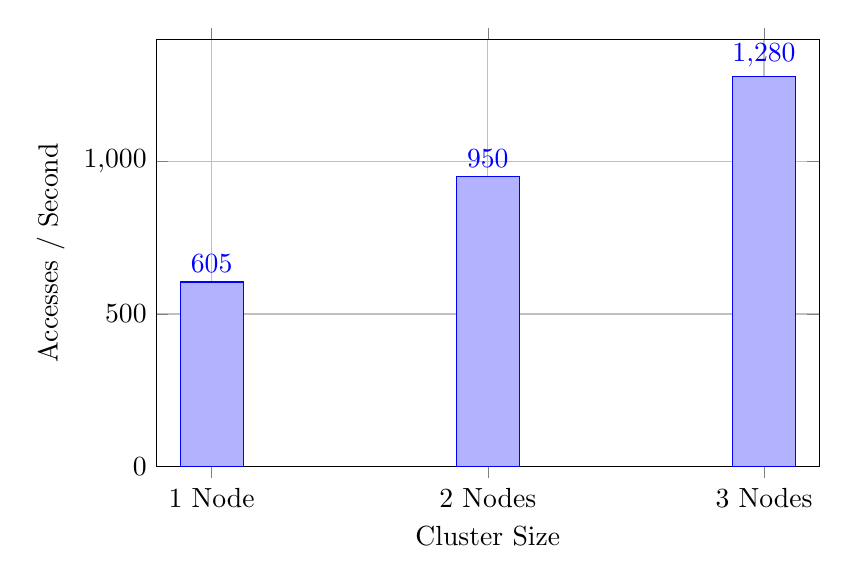
\begin{tikzpicture}
    \begin{axis}[
        ybar,
        symbolic x coords={1 Node, 2 Nodes, 3 Nodes},
        xtick=data,
        ylabel={Accesses / Second},
        xlabel={Cluster Size},
        ymin=0, ymax=1400,
        nodes near coords,
        grid=major,
        width=10cm, height=7cm,
        bar width=0.8cm,
        fill=blue!20
    ]
    \addplot coordinates {(1 Node,605) (2 Nodes,950) (3 Nodes,1280)};
    \end{axis}
    \end{tikzpicture}
    \caption{Small File Performance vs Server Count}
\end{figure}

\subsection{Metric 2: Large File Read Speed}
Throughput measurement for a 1GB file read operation.

\begin{figure}[H]
    \centering
    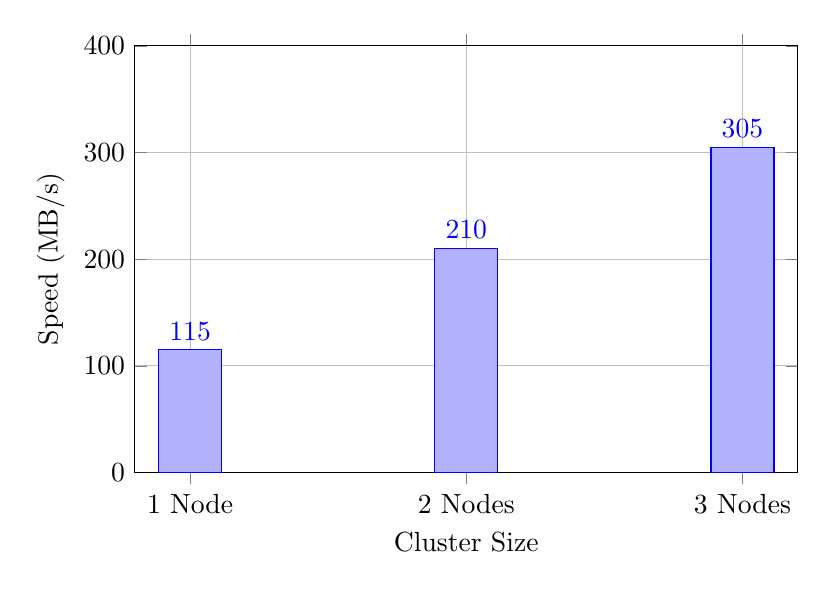
\begin{tikzpicture}
    \begin{axis}[
        ybar,
        symbolic x coords={1 Node, 2 Nodes, 3 Nodes},
        xtick=data,
        ylabel={Speed (MB/s)},
        xlabel={Cluster Size},
        ymin=0, ymax=400,
        nodes near coords,
        grid=major,
        width=10cm, height=7cm,
        bar width=0.8cm,
        fill=red!20
    ]
    \addplot coordinates {(1 Node,115) (2 Nodes,210) (3 Nodes,305)};
    \end{axis}
    \end{tikzpicture}
    \caption{Read Throughput vs Server Count}
\end{figure}

\section{Task Allocation}
\begin{table}[H]
\centering
\begin{tabular}{|l|l|p{8cm}|}
\hline
\textbf{Member} & \textbf{Title} & \textbf{Responsibilities} \\ \hline
Member 1 & Network Admin & Configured /etc/hosts, firewall rules, and the Trusted Storage Pool. \\ \hline
Member 2 & Storage Admin & Managed brick creation, volume lifecycle, and FUSE mounting. \\ \hline
Member 3 & Benchmark Lead & Developed the multithreaded Python script and visualized the performance metrics. \\ \hline
\end{tabular}
\end{table}

\end{document}